\documentclass[a4paper, 11pt]{report} % {{{
	\usepackage[utf8]{inputenc}
	\usepackage[T1]{fontenc}
	\usepackage[french]{babel}
	\usepackage{amsmath}
    \usepackage{amsfonts}
	\usepackage{nicefrac}
    \usepackage{graphicx}
    \usepackage{geometry}

    \geometry{left=3cm,right=3cm,top=4cm,bottom=3cm}

	% Renuméroter les section /sous sections joliement
    \renewcommand{\thesection}{\Roman{section} - }
    \renewcommand{\thesubsection}{\Alph{subsection}) }
    
    % "dx" et "dt" pour la dérivation
    \newcommand{\dx}{\mathrm{d}x}
    \newcommand{\dy}{\mathrm{d}y}
    \newcommand{\dt}{\mathrm{d}t}
    \newcommand{\dl}{\mathrm{d}l}

    \newcommand{\R}{\mathbb{R}}

    % des flèches plus longues pour les définitions de fonction
    \renewcommand{\mapsto}{\longmapsto}

    \title{L2 SPI --- Maths}
    \author{Mathieu Gaborit}
    \date{Novembre 2012}

% }}}
\begin{document}
    \maketitle

\section{Intégrales} % {{{

\subsection{$h(x) = \sqrt{\left|1-x\right|}$, pour $x\in[0, 2]$} % {{{

\paragraph{Sur $[0,1]$}
$1-x \geq 0$, donc $\sqrt{1-x}$ existe.

\paragraph{Sur $[1,2]$}
$1-x \leq 0$, mais $x-1\geq 0$ et $\left|1-x\right| = x-1$, donc $\sqrt{\left|1-x\right|} = \sqrt{x-1}$.

On peut donc redéfinir $h(x)$ de la manière suivante :

\[
h(x) = \sqrt{\left|1-x\right|} \Leftrightarrow\left\{
    \begin{array}{ll}
        \sqrt{1 - x} &\forall x\in[0,1]\\
        \sqrt{x - 1} &\forall x\in[1,2]
    \end{array}
    \right.
\]

On peut ainsi écrire l'intégrale comme une somme d'intégrales :

\[
\int_0^2h(x)\dx = \underbrace{\int_0^1\sqrt{1-x}\dx}_{(1)} + \underbrace{\int_1^2\sqrt{x-1}\dx}_{(2)}
\]

\paragraph{Résolution de l'intégrale $(1)$}

On procède par changement de variable :

\[ y = 1 - x, ~~ x = 1 - y, ~~ \dx = -\dy \]

On change ensuite les bornes :

\[ \begin{tabular}{c}
    1 - 0 = 1\\
    1 - 1 = 0
\end{tabular}
\]

On arrive donc à :

\begin{eqnarray*}
\int_0^1\sqrt{1-x}\dx & \Leftrightarrow & \int_1^0 - \sqrt{y}\dy\\
& \Leftrightarrow & \int_0^1y^{\nicefrac{1}{2}}\dy \\
& \Leftrightarrow & \left[y^{\nicefrac{3}{2}}\right]_0^1 \\
& \Leftrightarrow & \frac{1}{3}
\end{eqnarray*}

\paragraph{Résolution de l'intégrale $(2)$}

On procède là encore par changement de variable

\[ y = x - 1, ~~ x = y - 1, ~~ \dx = \dy \]

On change ensuite les bornes :

\[ \begin{tabular}{c}
    1 - 1 = 0\\
    2 - 1 = 1
\end{tabular}
\]

On arrive donc à :

\begin{eqnarray*}
\int_0^1\sqrt{1-x}\dx & \Leftrightarrow & \int_0^1 \sqrt{y}\dy\\
\end{eqnarray*}

Soit l'intégrale calculée juste au dessus, on peut donc calculer l'intégrale complète :

\begin{eqnarray*}
\int_0^2h(x)\dx & = & 2\times\int_0^1\sqrt{y}\dy\\
& = & 2\times \frac{2}{3}\\
& = & \frac{4}{3}
\end{eqnarray*}

% }}}

\subsection{$h(x) = \sqrt{\left|1-x\right|}$, pour $x\in[0, 2]$} % {{{

On cherche à calculer :

\[
I = \int_2^3\ln(x^2-1)\dx
\]

On commence par opérer une intégration par parties en posant :

\[
\left\{
\begin{array}{l}
u(x) = \ln(x^2-1)\\
v'(x) = 1
\end{array}
\right.
\Leftrightarrow
\left\{
\begin{array}{l}
u'(x) = \frac{2x}{x^2-1}\\ 
v(x) = x
\end{array}
\right.
\]

L'équation devient alors :

\begin{eqnarray*}
I & = & \left[x\ln(x^2-1)\right]_2^3 - \int_2^3\frac{2x^2}{x^2-1}\dx\\
& = & \left[x\ln(x^2-1)\right]_2^3 - \int_2^3\frac{2x^2 - 2 + 2}{x^2-1}\dx\\
& = & \left[x\ln(x^2-1)\right]_2^3 - 2\int_2^3\dx+2\int_2^3\frac{1}{x^2-1}\dx\\
& = & \underbrace{\left[x\ln(x^2-1)\right]_2^3 - 2\int_2^3\dx}_{(1)} + \underbrace{2\int_2^3\frac{1}{x^2-1}\dx}_{(2)}\\
\end{eqnarray*}

Si la partie $(1)$ se calcule sans souci, la partie $(2)$ est un peu plus compliquée.
Je me suis penché sur les développements possibles de $\nicefrac{1}{x^2-1}$ et ai trouvé une formule utilisant limités
et me permettant de réduire ainsi :

\begin{eqnarray*}
(2) & \Leftrightarrow & 2\int_2^3\frac{1}{2(x-1)}-\frac{1}{2(x+1)}\dx\\
& \Leftrightarrow & \int_2^3\frac{1}{x-1}-\frac{1}{x+1}\dx\\
& \Leftrightarrow & \left[\ln(x-1)\right]_2^3-\left[\ln(x+1)\right]_2^3\\
\end{eqnarray*}

On ré-injecte alors dans notre équation et on a :

\begin{eqnarray*}
I & = & \left[x\ln(x^2-1)\right]_2^3 - 2\int_2^3\dx + \left[\ln(x-1)\right]_2^3-\left[\ln(x+1)\right]_2^3\\
& = & 3\ln(2^3)-2\ln(3)-2-\ln(2)+\ln(2^2)-\ln(3)\\
& = & 9\ln(2) - 2\ln(3)-2-\ln(2)+2\ln(2)-\ln(3)\\
& = & 10\ln(2) - 3\ln(3) -2\\
& \approx & 1.63563
\end{eqnarray*}


% }}}

% }}}
\section{Masse d'un fil} % {{{

On commence par écrire une fonction de $\R$ dans $\R^2$ décrivant la courbe, à parcourir pour $x \in [0, 1]$ :

\[
\begin{array}{llll}
    \gamma : & \R & \longrightarrow & \R^2\\
    & t & \mapsto & \begin{pmatrix}t\\t^2\end{pmatrix}
\end{array}
\]

La dérivé de $\gamma(t)$ est alors :

\[\gamma'(t) = \begin{pmatrix}1\\2t\end{pmatrix}\]

Et on calculera facilement la norme de $\gamma'(t)$ :

\begin{eqnarray*}
\lVert\gamma'(t)\rVert & = & \sqrt{1^2 + (2t)^2}\\
& = & \sqrt{1 + 4t^2}
\end{eqnarray*}

On définit par ailleurs une fonction décrivant la densité au point de paramètre $x$ telle que :

\[
\begin{array}{c}
\rho(x, y) = \sqrt{1+4x^2}\\
\rho(\gamma(t)) = \sqrt{1+4x^2}
\end{array}
\]

Reste à écrire l'intégrale curviligne permettant de calculer la masse $M$ :

\begin{eqnarray*}
M & = & \int_0^1\rho(\gamma(t))\times\lVert\gamma'(t)\rVert\dt\\
& = & \int_0^1\sqrt{1+4t^2}\cdot\sqrt{1+4t^2}\dt\\
& = & \int_0^1\dt + \int_0^14t^2\dt\\
& = & 1 + \frac{4}{3}\left[x^3\right]_0^1\\
& = & \frac{3}{3} + \frac{4}{3}\\
M & = & \frac{7}{3}
\end{eqnarray*}

% }}}
\section{Centre de gravité d'une courbe homogène} % {{{

% explications {{{
Il s'agit d'une courbe d'équation 

\begin{equation}
    \gamma(t) = 
    \begin{pmatrix}
        \cos(t)(1+\cos(t))\\
        \sin(t)(1+\cos(t))
    \end{pmatrix}
\end{equation}

On commence par dériver ladite équation (on en aura besoin ensuite) :

\begin{eqnarray*}
\gamma'(t) & = &
        \begin{pmatrix}
            \gamma_x'\\
            \gamma_y'
        \end{pmatrix}\\
& = &   \begin{pmatrix}
            -\sin(t)(1+\cos(t))-\sin(t)\cos(t)\\
            \cos(t)(1+\cos(t)) - \sin^2(t)
        \end{pmatrix}\\
& = &   \begin{pmatrix}
            -\sin(t) - 2\sin(t)\cos(t)
            \cos(t)+\cos^2(t)-sin^(t)
        \end{pmatrix}\\
& = &   \begin{pmatrix}
            -\sin(t) - \sin(2t)
            \cos(t) +\cos(2t)
        \end{pmatrix}
\end{eqnarray*}

Les deux simplifications entre les deux dernières lignes sont les suivantes :

\begin{eqnarray*}
    \cos^2(t)-\sin^2(t) & = & \cos(t)\cos(t)-\sin(t)\sin(t)\\
    & = & \cos(2t)\\
    2\sin(t)\cos(t) = \sin(2t)
\end{eqnarray*}

On aura aussi besoin de la norme de $\gamma'$ :

\[
    \lVert\gamma'(t)\rVert = \sqrt{\gamma'^2_x + \gamma'^2_y}
\]

On calculera les deux parties de la racines séparément.

\begin{eqnarray*}
    \left[-\sin(t)-\sin(2t)\right]^2 & = & (-1)^2\times\left[\sin(t)+\sin(2t)\right]^2\\
                                    & = & \sin^2(t)+2\sin(t)\sin(2t)+\sin^2(2t)\\
    \left[\cos(t)+\cos(2t)\right]^2 & = & \cos^2(t)+2\cos(t)\cos(2t)+\cos^2(2t)\\
\end{eqnarray*}


Reste à sommer le tout :

\begin{eqnarray*}
    \lVert\gamma'(t)\rVert^2 & = & \gamma'^2_x + \gamma'^2_y\\
    & = & \sin^2(t)+2\sin(t)\sin(2t)+\sin^2(2t) + \cos^2(t)+2\cos(t)\cos(2t)+\cos^2(2t)\\
    & = & \underbrace{\sin^2(t) + \cos^2(t)}_{=1} + 2\underbrace{\left[\sin(t)\sin(2t) +\cos(t)\cos(2t)\right]}_{=\cos(t)\mathrm{~(formules~de~transformation~somme-produit)}}+\underbrace{\cos^2(2t)+\sin^2(2t)}_{=1}\\
    \lVert\gamma'(t)\rVert & = &\sqrt{2+2\cos(t)}\\
\end{eqnarray*}

On peut ensuite simplifier ainsi (seulement parce que pour $t\in\left[0,\nicefrac{\pi}{2}\right],~\cos\left(\nicefrac{t}{2}\right) \geq 0$) :

\begin{eqnarray*}
    \lVert\gamma'(t)\rVert & = & \sqrt{2+2\cos(t)}\\
                           & = & \sqrt{2 + 2\cos\left(\frac{t}{2} +\frac{t}{2} \right)}\\
                           & = & \sqrt{2 + 2\left[2\cos^2\left(\frac{t}{2}\right)-1\right]}\\
                           & = & \sqrt{2 - 2 + 4\cos^2\left(\frac{t}{2}\right)}\\
                           & = & \sqrt{4\cos^2\left(\frac{t}{2}\right)}\\
                           & = & 2\cos\left(\frac{t}{2}\right)
\end{eqnarray*}

% }}}

\subsection{Calcul de la masse} % {{{

On a la formule suivante :

\[
    M = \int_\gamma\rho(x,y)\dl = \int_0^{\nicefrac{\pi}{2}}\rho(\gamma(t))\lVert\gamma'(t)\rVert\dt
\]


Ici, on est dans le cas d'une courbe homogène, donc $\forall x,y$, $\rho(x,y)=Cste=\rho_0$ :

On peut alrs écrire :

\begin{eqnarray*}
    M & = & \int_0^{\nicefrac{\pi}{2}}\rho_0\lVert\gamma'(t)\rVert\dt\\
      & = & \rho_0\int_0^{\nicefrac{\pi}{2}}2\cos\left(\frac{t}{2}\right)\dt\\
      & = & 2\rho_0\left[2\sin\left(\frac{t}{2}\right)\right]_0^{\nicefrac{\pi}{2}}\\
      & = & 4\rho_0\left(\frac{\sqrt{2}}{2}-0\right)\\
      & = & 2\rho_0\sqrt{2}
\end{eqnarray*}

On prendra dans la suite $\rho_0 = 1$ donc $M = 2\sqrt{2}$.

% }}}
\subsection{Calcul du centre de gravité} % {{{

On cherche désormais à calculer les coordonnées du centre de gravité $C$ de la courbe telles que
\[C = \begin{pmatrix}C_x\\C_y\end{pmatrix} = 
        \begin{pmatrix}
            \frac{1}{M}\int_\gamma\gamma_x\rho(x,y)\dl\\
            \frac{1}{M}\int_\gamma\gamma_y\rho(x,y)\dl
        \end{pmatrix} = 
        \begin{pmatrix}
            \frac{\rho_0}{M}\int_0^{\nicefrac{\pi}{2}}\cos(t)(1+\cos(t))\lVert\gamma'(t)\rVert\dt\\
            \frac{\rho_0}{M}\int_0^{\nicefrac{\pi}{2}}\sin(t)(1+\cos(t))\lVert\gamma'(t)\rVert\dt
        \end{pmatrix}
\]

\paragraph{Calcul de $C_x$} % {{{
Il s'agit de simplifier l'expression de $C_x$ en la mettant sous la forme d'une somme de sinus et/ou cosinus.

\begin{eqnarray*}
C_x & = & \frac{1}{M}\int_0^{\nicefrac{\pi}{2}}\cos(t)(1+\cos(t))\lVert\gamma'(t)\rVert\dt\\
    & = & \frac{2}{2\sqrt{2}}\int_0^{\nicefrac{\pi}{2}}\left(\cos(t)+\cos^2(t)\right)\cos\left(\frac{t}{2}\right)\dt\\
    & = & \frac{2}{2\sqrt{2}}\int_0^{\nicefrac{\pi}{2}}\cos(t)\cos\left(\frac{t}{2}\right)+\cos^2(t)\cos\left(\frac{t}{2}\right)\dt\\
    & = & \frac{2}{2\sqrt{2}}\int_0^{\nicefrac{\pi}{2}}
        \frac{1}{2}\cos\left(\frac{3t}{2}\right)+\frac{1}{2}\cos\left(\frac{t}{2}\right)+
        \frac{1}{2}\cos\left(\frac{t}{2}\right) + \frac{1}{4}\cos\left(\frac{5t}{2}\right)+\frac{1}{4}\cos\left(\frac{3t}{2}\right)\\
    & = & \frac{2}{2\sqrt{2}}\int_0^{\nicefrac{\pi}{2}}
        \frac{3}{4}\cos\left(\frac{3t}{2}\right)+\cos\left(\frac{t}{2}\right)+ \frac{1}{4}\cos\left(\frac{5t}{2}\right)\\
    & = & \frac{1}{2\sqrt{2}}\int_0^{\nicefrac{\pi}{2}}
        \frac{3}{2}\cos\left(\frac{3t}{2}\right)+2\cos\left(\frac{t}{2}\right)+ \frac{1}{2}\cos\left(\frac{5t}{2}\right)\\
    & = & \frac{1}{2\sqrt{2}}\left[
            \frac{3}{2}\int_0^{\nicefrac{\pi}{2}}\cos\left(\frac{3t}{2}\right)+
            2\int_0^{\nicefrac{\pi}{2}}\cos\left(\frac{t}{2}\right)+
            \frac{1}{2}\int_0^{\nicefrac{\pi}{2}}\cos\left(\frac{5t}{2}\right)
        \right]\\
    & = & \frac{1}{2\sqrt{2}}\left[
        \frac{3}{2}\times\frac{2}{3}\left[\sin\left(\frac{3t}{2}\right)\right]_0^{\nicefrac{\pi}{2}}+
        4\left[\sin\left(\frac{t}{2}\right)\right]_0^{\nicefrac{\pi}{2}}+
        \frac{1}{2}\times\frac{2}{5}\left[\sin\left(\frac{5t}{2}\right)\right]_0^{\nicefrac{\pi}{2}}
        \right]\\
    & = & \frac{1}{2\sqrt{2}}\left(
        \frac{\sqrt{2}}{2}+
        4\times\frac{\sqrt{2}}{2}-
        \frac{1}{5}\times\frac{\sqrt{2}}{2}
        \right)\\
C_x & = & \frac{6}{5}
\end{eqnarray*}

% }}}

\paragraph{Calcul de $C_y$} % {{{

Il s'agit de simplifier l'expression de $C_y$ en la mettant sous la forme d'une somme de sinus et/ou cosinus.

\begin{eqnarray*}
C_y & = & \frac{1}{M}\int_0^{\nicefrac{\pi}{2}}\sin(t)(1+\cos(t))\lVert\gamma'(t)\rVert\dt\\
    & = & \frac{2}{2\sqrt{2}}\int_0^{\nicefrac{\pi}{2}}\left(\sin(t)+\sin(t)\cos(t)\right)\cos\left(\frac{t}{2}\right)\dt\\
    & = & \frac{2}{2\sqrt{2}}\int_0^{\nicefrac{\pi}{2}}\sin(t)\cos\left(\frac{t}{2}\right)+\sin(t)\cos(t)\cos\left(\frac{t}{2}\right)\dt\\
    & = & \frac{2}{2\sqrt{2}}\int_0^{\nicefrac{\pi}{2}}
        \frac{1}{2}\left[\sin\left(\frac{3t}{2}\right)+\sin\left(\frac{t}{2}\right)\right]+
        \frac{1}{2}\sin(t)\left[\cos\left(\frac{3t}{2}\right)+\cos\left(\frac{t}{2}\right)\right]\dt\\
    & = & \frac{2}{2\sqrt{2}}\int_0^{\nicefrac{\pi}{2}}
        \frac{1}{2}\left[\sin\left(\frac{3t}{2}\right)+\sin\left(\frac{t}{2}\right)\right]+
        \frac{1}{2}\sin(t)\cos\left(\frac{3t}{2}\right)+
        \frac{1}{2}\sin(t)\cos\left(\frac{t}{2}\right)\dt\\
    & = & \frac{1}{2\sqrt{2}}\int_0^{\nicefrac{\pi}{2}}
        \left[\sin\left(\frac{3t}{2}\right)+\sin\left(\frac{t}{2}\right)\right]+
        \sin(t)\cos\left(\frac{3t}{2}\right)+
        \sin(t)\cos\left(\frac{t}{2}\right)\dt\\
    & = & \frac{1}{2\sqrt{2}}\int_0^{\nicefrac{\pi}{2}}
        \left[\sin\left(\frac{3t}{2}\right)+\sin\left(\frac{t}{2}\right)\right]+
        \sin(t)\cos\left(\frac{3t}{2}\right)+
        \frac{1}{2}\left[\sin\left(\frac{3t}{2}\right)+\sin\left(\frac{t}{2}\right)\right]\dt\\
    & = & \frac{1}{2\sqrt{2}}\int_0^{\nicefrac{\pi}{2}}
        \frac{3}{2}\sin\left(\frac{3t}{2}\right)+
        \frac{3}{2}\sin\left(\frac{t}{2}\right)+
        \sin(t)\cos\left(\frac{3t}{2}\right)\dt\\
    & = & \frac{1}{2\sqrt{2}}\int_0^{\nicefrac{\pi}{2}}
        \frac{3}{2}\sin\left(\frac{3t}{2}\right)+
        \frac{3}{2}\sin\left(\frac{t}{2}\right)+
        \frac{1}{2}\left[\sin\left(\frac{5t}{2}\right)-\sin\left(\frac{t}{2}\right)\right]\dt\\
    & = & \frac{3}{4\sqrt{2}}\left[
        \int_0^{\nicefrac{\pi}{2}}
        \sin\left(\frac{3t}{2}\right)\dt+
        \int_0^{\nicefrac{\pi}{2}}
        \sin\left(\frac{t}{2}\right)\dt
        \right]+
        \frac{1}{4\sqrt{2}}
        \left[
        \int_0^{\nicefrac{\pi}{2}}
        \sin\left(\frac{5t}{2}\right)\dt-
        \int_0^{\nicefrac{\pi}{2}}
        \sin\left(\frac{t}{2}\right)\dt
        \right]\\
    & = & \frac{3}{4\sqrt{2}}\left[
        -\frac{2}{3}
        \left[
        \cos\left(\frac{3t}{2}\right)+
        \right]_0^{\nicefrac{\pi}{2}}
        -2
        \left[
        \cos\left(\frac{t}{2}\right)
        \right]_0^{\nicefrac{\pi}{2}}
        \right]+
        \frac{1}{2\sqrt{2}}
        \left[
        -\frac{1}{5}
        \left[
        \cos\left(\frac{5t}{2}\right)-
        \right]_0^{\nicefrac{\pi}{2}}
        +\left[
        \cos\left(\frac{t}{2}\right)
        \right]_0^{\nicefrac{\pi}{2}}
        \right]\\
    & = & \frac{3}{4\sqrt{2}}\left[
        -\frac{2}{3}
        \left(
            -\frac{\sqrt{2}}{2}-1
        \right)
        -2
        \left(
            \frac{\sqrt{2}}{2}-1
        \right)
        \right]+
        \frac{1}{2\sqrt{2}}
        \left[
        -\frac{1}{5}
        \left(
            -\frac{\sqrt{2}}{2} - 1
        \right)
        +\frac{\sqrt{2}}{2} - 1
        \right]\\
    & = & \frac{3}{4\sqrt{2}}\left[
            -\frac{\sqrt{2}}{3}-\frac{2}{3}
            -\sqrt{2} + 2
        \right]+
        \frac{1}{2\sqrt{2}}\left[
            -\frac{\sqrt{2}}{10} + \frac{1}{5}
            +\frac{\sqrt{2}}{2} - 1
        \right]\\
    C_y & \approx & 0.931
\end{eqnarray*}
% }}}

\[
    C = 
    \begin{pmatrix}
        \nicefrac{6}{5}\\
        0.931\ldots
    \end{pmatrix}
\]
% }}}
% }}}
\section{Travail sur un triangle} % {{{

Pour mieux saisir le sujet, on commence par un petit schéma :

\begin{figure}[!h]
    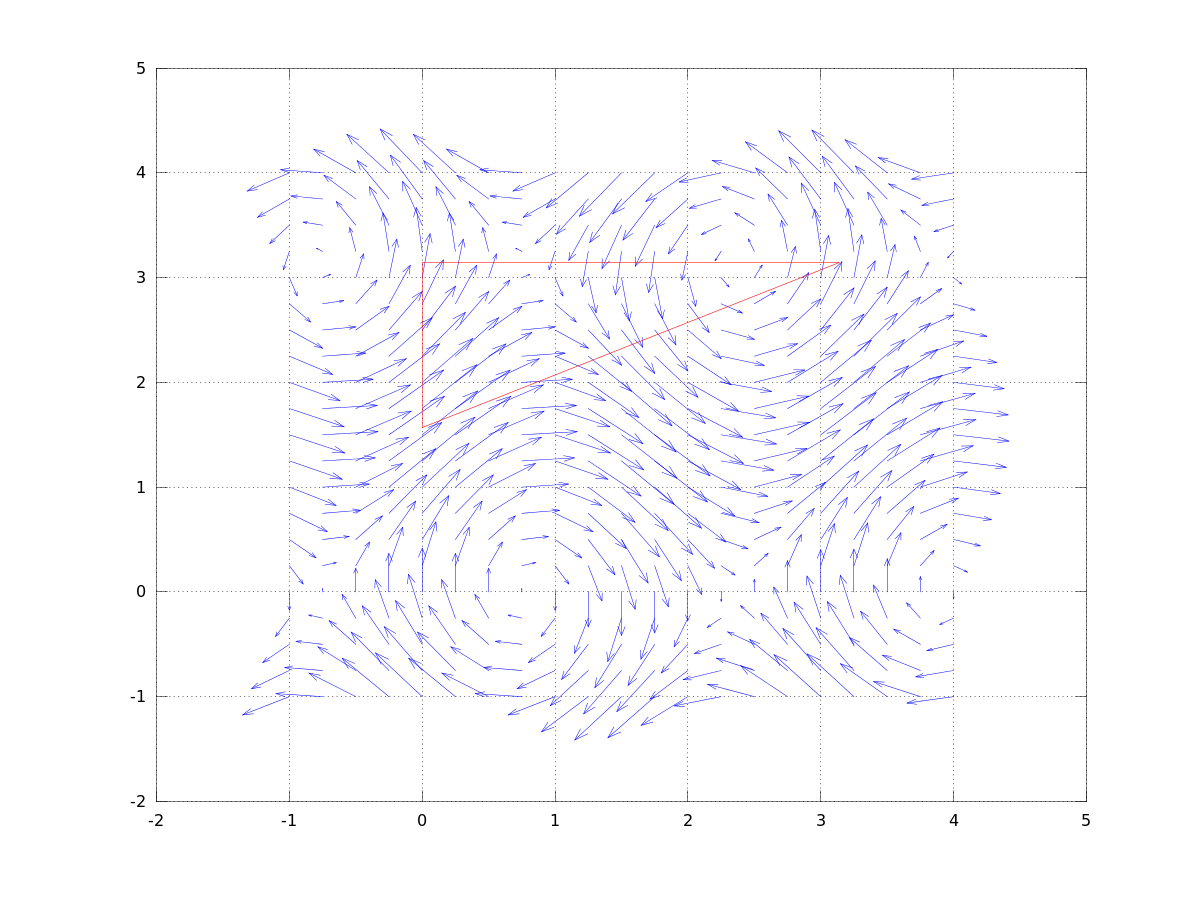
\includegraphics[width=15cm]{exo4.png}
    \caption{\label{fig_exo4} Le champ de vecteurs (en bleu) et le triangle (en rouge)}
\end{figure}

On a l'expression de notre champ de force tel que :

\[
F(x, y) =
\begin{pmatrix}
\sin(y)\\
\cos(2x)
\end{pmatrix}
\]

On cherche donc à calculer le travail de la force appliquée par ce champ sur un corps parcourant le triangle rouge
composé des points $A(0, \pi)$, $B(\pi,\pi)$ et $C(0,\nicefrac{\pi}{2})$. On parcourt le triangle dans l'ordre $A
\rightarrow B \rightarrow C \rightarrow A$.

On sait le que le travail total $W$ est égal à la somme des travaux sur $[AB]$, $[BC]$ et $[CA]$ :

\[ W = W_{AB} + W_{BC} + W_{CA} \]

On peut définir une fonction $\gamma(t)$ pour chaque segment de droite en fonction d'un paramètre $t$ variant entre $0$
et $\pi$. Pour deux points $X(X_x, X_y)$ et $Y(Y_x, Y_y)$ et le segment $X \rightarrow Y$, on aura :

\[
\gamma_{XY} =
\begin{pmatrix}
\nicefrac{Y_x - X_x}{\pi}t+X_x\\
\nicefrac{Y_y - X_y}{\pi}t+X_y
\end{pmatrix}
\]

On peut ensuite définir pour chaque segment l'action de $F$ sur ce segment $F(\gamma(t))$ et la dérivée $\gamma'(t)$ de
$\gamma(t)$.

On a alors :

\begin{eqnarray*}
\gamma_{AB}(t) =
\begin{pmatrix}
t\\
\pi
\end{pmatrix} &
F_{\gamma_{AB}} = 
\begin{pmatrix}
\sin(\pi)\\
\cos(2t)
\end{pmatrix} &
\gamma'_{AB}(t) =
\begin{pmatrix}
1\\
0
\end{pmatrix}\\ % NEWLINE
\gamma_{BC}(t) =
\begin{pmatrix}
-t+\pi\\
-\nicefrac{t}{2}+\pi
\end{pmatrix} &
F_{\gamma_{BC}} = 
\begin{pmatrix}
\sin(-\nicefrac{t}{2}+\pi)\\
\cos(-2t)
\end{pmatrix} &
\gamma'_{BC}(t) =
\begin{pmatrix}
-1\\
-\nicefrac{1}{2}
\end{pmatrix}\\ % NEWLINE
\gamma_{CA}(t) =
\begin{pmatrix}
0\\
\nicefrac{t}{2} +\nicefrac{\pi}{2}
\end{pmatrix} &
F_{\gamma_{CA}} = 
\begin{pmatrix}
\sin(\nicefrac{t}{2} +\nicefrac{\pi}{2})\\
\cos(0)
\end{pmatrix} &
\gamma'_{CA}(t) =
\begin{pmatrix}
0\\
\nicefrac{1}{2}
\end{pmatrix}
\end{eqnarray*}

\paragraph{$W_{AB}$}

\begin{eqnarray*}
W_{AB} & = &
\int_0^\pi
\begin{pmatrix}
\sin(\pi)\\
\cos(2t)
\end{pmatrix}
\cdot
\begin{pmatrix}
1\\
0
\end{pmatrix}
\dt\\
& = & \int_0^\pi\sin(\pi)\dt\\
& = & 0
\end{eqnarray*}

\paragraph{$W_{BC}$}

\begin{eqnarray*}
W_{BC} & = &
\int_0^\pi
\begin{pmatrix}
\sin(-\nicefrac{t}{2}+\pi)\\
\cos(-2t)
\end{pmatrix} 
\cdot
\gamma'_{BC}(t) =
\begin{pmatrix}
-1\\
-\nicefrac{1}{2}
\end{pmatrix}
\dt\\
& = & -\int_0^\pi\sin(-\nicefrac{t}{2}+\pi)\dt-\int_0^\pi\cos(-2t)\dt\\
& = & 2\left[\cos\left(-\frac{t}{2}+\pi\right)\right]_0^\pi - \frac{1}{4}\left[\sin(-2t)\right]_0^\pi\\
& = & -2
\end{eqnarray*}

\paragraph{$W_{CA}$}

\begin{eqnarray*}
W_{CA} & = &
\int_0^\pi
\begin{pmatrix}
\sin(\nicefrac{t}{2} +\nicefrac{\pi}{2})\\
\cos(0)
\end{pmatrix}
\cdot
\gamma'_{CA}(t) =
\begin{pmatrix}
0\\
\nicefrac{1}{2}
\end{pmatrix}
\dt\\
& = & \frac{1}{2}\int_0^\pi\cos(0)\dt\\
& = & \frac{\pi}{2}
\end{eqnarray*}


On somme alors :

\begin{eqnarray*}
W & = & W_{AB} + W_{BC} + W_{CA}\\
& = & \frac{\pi}{2} - 2
\end{eqnarray*}

% }}}
\section{Travail d'un champ de force} % {{{

\begin{figure}[!h]
    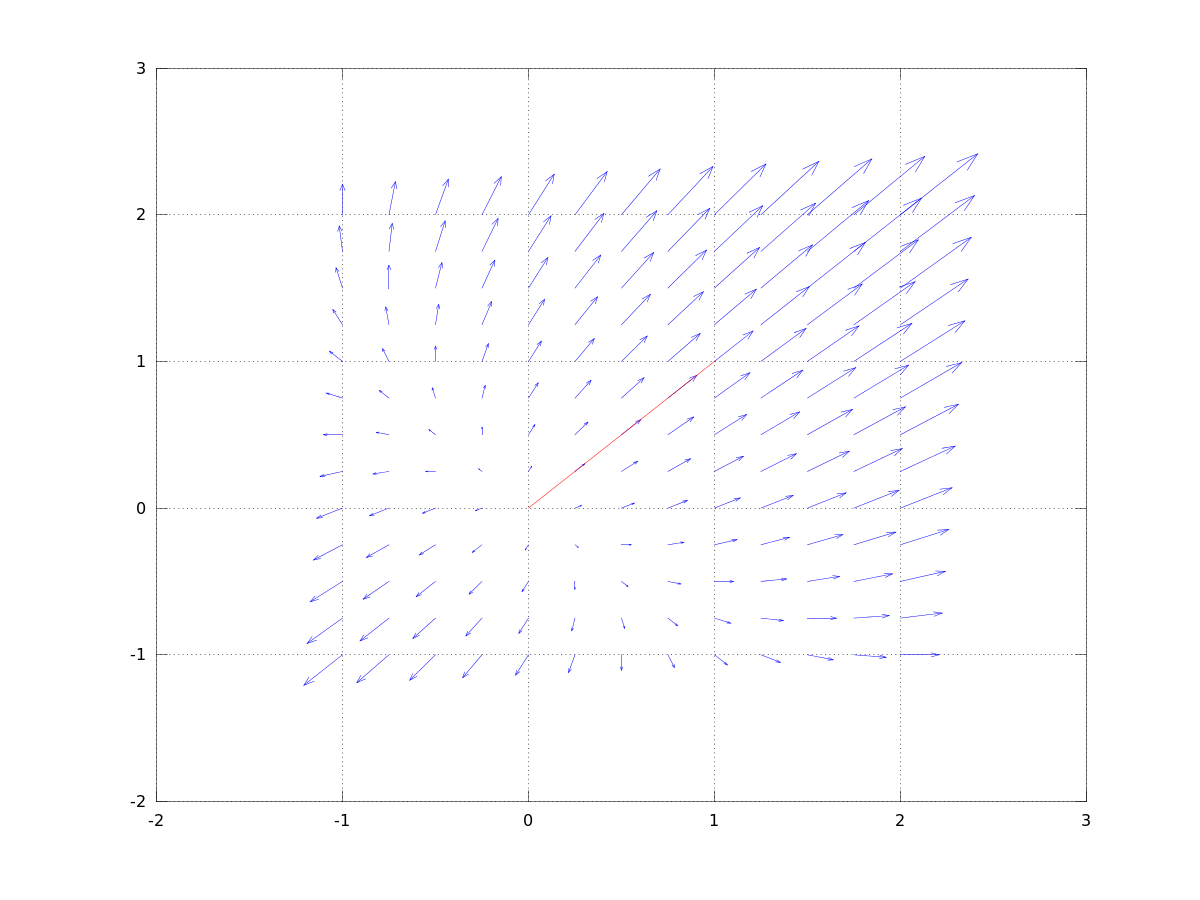
\includegraphics[width=15cm]{exo5.png}
    \caption{\label{fig_exo5} Le champ de vecteurs (en bleu) et la droite de déplacement (en rouge)}
\end{figure}
Afin de mieux visualiser le problème, on commence par tracer le champ de vecteurs (en bleu) et la droite sur laquelle on se
déplace (en rouge), la figure finale est disponible en figure~\ref{fig_exo5}.

L'équation de la courbe de déplacement est : $y(t) = \nicefrac{\Delta y}{\Delta x}t = \frac{1}{1}t = t$, on peut la
ré-écrire sous la forme d'une fonction de $\R$ dans $\R^2$ : 

\[
\begin{array}{llll}
    \gamma : & \R & \longrightarrow & \R^2\\
    & t & \mapsto & \begin{pmatrix}t\\t\end{pmatrix}
\end{array}
\]

Le déplacement s'effectue dans un champ de force (\textit{i.e.} un champ de vecteurs) d'équation :

\[
\begin{array}{llll}
    F : & \R^2 & \longrightarrow & \R^2\\
    & \begin{pmatrix}
        x\\
        y
      \end{pmatrix} & \mapsto &
      \begin{pmatrix}
        2x+y\\
        2y+x
      \end{pmatrix}
\end{array}
\]

On calcule aisément $F(\gamma(t))$ pour $t\in[0,1]$ :

\[
F(\gamma(t)) = \begin{pmatrix}
3t\\
3t
\end{pmatrix}
\]

On calcule de même $\gamma'(t)$ :

\[
\gamma'(t) = \begin{pmatrix}
1\\
1
\end{pmatrix}
\]

Enfin, calculer le travail du champ de force revient à intégrer pour $t$ allant de $0$ à $1$ le produit scalaire de
$F(\gamma(t))$ et de $\gamma'(t)$ :

\begin{eqnarray*}
    \int_0^1
    \begin{pmatrix}
    3t\\
    3t
    \end{pmatrix}
    \cdot
    \begin{pmatrix}
    1\\
    1
    \end{pmatrix}
    \dt
    & = & 2\int_0^13t\dt\\
    & = & 6\int_0^1t\dt\\
    & = & 6\left[\frac{1}{2}t^2\right]_0^1\\
    & = & 3
\end{eqnarray*}

Cette quantité étant positive, on en déduit que le travail est globalement moteur.

% }}}
\section{Equations différentielles} % {{{

\subsection{$x' + x = e^{-t}, x(0) = 0$} % {{{

\begin{equation}
x' + x = e^{-t}
\label{equa_diff_1}
\end{equation}

C'est une équation différentielle du premier ordre, la solution de l'équation homogène (sans second membre) est donc :

\[
S_h = \left\{\lambda e^{-t} + g_0, \lambda\in\R\right\}
\]

Avec $g_0$ une solution particulière.

\paragraph{Recherche d'une solution particulière}
On a $x' = x = e^{-t}$, soit $x' + ax = P(t)e^{rt}$ avec $P(t) = 1, a = 1, r = -1$.

On remarque que $a=-r$, on aura donc une solution particulière à l'équation (\ref{equa_diff_1}) de la forme :

\[ g_0 : t \mapsto Q(t)e^{-t} \]

où $Q(t)$ est un polynôme tel que $\mathrm{deg}Q = \mathrm{deg}P + 1$, $Q(t)$ sera donc de la forme :

\[ Q(t) = \alpha t + \beta \]

d'où :

\[
\begin{array}{c}
g_0 : t\mapsto (\alpha x + \beta)e^{-t}\\
g_0' : t \mapsto \alpha e^{-t} - \alpha te^{-t} - \beta e^{-t}
\end{array}
\]

$g_0$ étant solution de (\ref{equa_diff_1}), on remplace pour déterminer les constantes $\alpha$ et $\beta$ :

\[
\alpha e^{-t} + (\beta - \beta)e^{-t} + (\alpha - \alpha)te{-t} = e^{-t}
\]

On remarque que tout se simplifie, et qu'il ne reste plus que $\alpha = 1$ (après division par $e^{-t}$.
$\beta$ n'a pas d'importance et peut prendre d'importe quelle valeur, ici, nous choisirons 0.

\[ g_0 : t\mapsto te^{-t} \]

Et donc, la solution générale est :

\[ S_g = \left\{\lambda e^{-t} + te^{-t}, \lambda\in\R\right\} \]

\paragraph{Solution unique}
On fixe enfin la constante $\lambda$ au regard des conditions initiales :

\begin{eqnarray*}
    x(0) = 0 & \Rightarrow & \lambda e^0 = 0\\
    & \Rightarrow & \lambda = 0
\end{eqnarray*}

Ce qui nous donne, pour solution finale :

\[
x : t \mapsto te^{-t}
\]
% }}}
\subsection{$x'' - 4x = 0$} % {{{

\begin{equation}
x'' - 4x = 0
\label{equa_diff_2}
\end{equation}

Les conditions initiales sont les suivantes :

\[
\left\{\begin{array}{l}
x(0) = 1\\
x'(0) = 0
\end{array}\right.
\]

C'est une équation différentielle du second ordre, on calcule le discriminant de l'équation caractéristique (\ref{ec_1})
pour connaitre la forme de la solution :

\begin{equation}
X^2 - 4 = 0
\label{ec_1}
\end{equation}

\begin{eqnarray*}
    \Delta & = & 16\\
    r_0 & = & \frac{-\sqrt{\Delta}}{2}\\
    & = & -2\\
    r_1 & = & \frac{\sqrt{\Delta}}{2}\\
    & = & 2\\
\end{eqnarray*}

\[
S_h = \left\{Ae^{-2t} + Be^{2t} + g_0,~A,B\in\R\right\}
\]

Avec $g_0$ une solution particulière.

\paragraph{Recherche d'une solution particulière}

Le second membre de l'équation est une constante, la solution en sera donc une aussi.

On prend $g_0$ égale au second membre, soit $g_0 = 0$, on a alors $g_0' = g_0'' = 0$.

Pour vérification on remplace dans l'équation~\ref{equa_diff_2} :

\[
0 - 4\times0 = 0
\]

Notre solution particulière est donc cohérente

Notre solution générale ressemble alors à :

\[
S_g = \left\{Ae^{-2t} + Be^{2t},~A,B\in\R\right\}
\]

La dérivée de cette solution générale est l'ensemble des fonctions

\[
S_g' = \left\{-2Ae^{-2t} + 2Be^{2t},~A,B\in\R\right\}
\]

\paragraph{Solution unique}
On fixe enfin les constantes $A$ et $B$ avec les conditions initiales :

\begin{eqnarray*}
\left\{\begin{array}{l}
x(0) = 1\\
x'(0) = 0
\end{array}\right. & \Leftrightarrow &
\left\{\begin{array}{l}
Ae^0 + Be^0 = 1\\
-2Ae^0 - 2Be^0 = 0
\end{array}\right.\\
& \Leftrightarrow &                     % NEWLINE
\left\{\begin{array}{ll}
A + B = 1 & (L_1)\\
-2A - 2B = 0 & (L_2)
\end{array}\right.\\
& \Leftrightarrow &                     % NEWLINE
\left\{\begin{array}{ll}
A = 1 - B & (L_1)\\
4B = 2 & (L_3 \leftarrow L_2 + 2L_1)
\end{array}\right.\\
& \Leftrightarrow &                     % NEWLINE
\left\{\begin{array}{ll}
A = \frac{1}{2} & (L_1)\\
B = \frac{1}{2} & (L_3)
\end{array}\right.\\
\end{eqnarray*}

Ce qui nous donne, pour solution finale :

\[
x : t \mapsto \frac{1}{2}e^{-2t} + \frac{1}{2}e^{2t}
\]
% }}}
\subsection{$x'' + 4x' + 4x = 1$} % {{{

\begin{equation}
x'' + 4x' + 4x = 1
\label{equa_diff_3}
\end{equation}

Les conditions initiales sont les suivantes :

\[
\left\{\begin{array}{l}
x(0) = 1\\
x'(0) = 0
\end{array}\right.
\]

C'est une équation différentielle du second ordre, on calcule le discriminant de l'équation caractéristique (\ref{ec_2})
pour connaitre la forme de la solution :

\begin{equation}
X^2 + 4X + 4 = 0
\label{ec_2}
\end{equation}

\begin{eqnarray*}
    \Delta & = & 0\\
    r & = & \frac{-4}{2}\\
    & = & -2\\
\end{eqnarray*}

\[
S_h = \left\{Ae^{-2t} + Bte^{-2t} + g_0,~A,B\in\R\right\}
\]

Avec $g_0$ une solution particulière.

\paragraph{Recherche d'une solution particulière}

Le second membre de l'équation est une constante, la solution en sera donc une aussi.

Si $g_0$ est constante, alors ses dérivées \textit{n-ième} seront nulles, $g_0$ étant avant tout solution de
(\ref{equa_diff_3}), on peut écrire :

\[ 0 + 4\times0 + 4\times g_0 = 1 \]

On aura donc :

\[
g_0 = \frac{1}{4}
\]


La solution générale ressemble alors à :

\[
S_g = \left\{Ae^{-2t} + Bte^{-2t} + \frac{1}{4},~A,B\in\R\right\}
\]

La dérivée de cette solution générale est l'ensemble des fonctions

\[
S_g' = \left\{-2Ae^{-2t} + Be^{-2t} - 2Bte^{-2t},~A,B\in\R\right\}
\]

\paragraph{Solution unique}
On fixe enfin les constantes $A$ et $B$ avec les conditions initiales :

\begin{eqnarray*}
\left\{\begin{array}{l}
x(0) = 1\\
x'(0) = 0
\end{array}\right. & \Leftrightarrow &
\left\{\begin{array}{l}
Ae^0 + \frac{1}{4} = 1\\
-2Ae^0 + Be^0 = 0
\end{array}\right.\\
& \Leftrightarrow &                     % NEWLINE
\left\{\begin{array}{ll}
A = \frac{3}{4} & (L_1)\\
-2A + B = 0 & (L_2)
\end{array}\right.\\
& \Leftrightarrow &                     % NEWLINE
\left\{\begin{array}{ll}
A = \frac{3}{4} & (L_1)\\
B = 2\times\frac{3}{4} & (L_2)
\end{array}\right.\\
& \Leftrightarrow &                     % NEWLINE
\left\{\begin{array}{ll}
A = \nicefrac{3}{4} & (L_1)\\
B = \nicefrac{3}{2} & (L_2)
\end{array}\right.\\
\end{eqnarray*}

Ce qui nous donne, pour solution finale :

\[
x : t \mapsto \frac{3}{4}e^{-2t} - \frac{3}{2}te^{-2t} + \frac{1}{4}
\]
% }}}
\subsection{$x'' -3x' + 2x = e^{-t}$} % {{{

\begin{equation}
x'' -3x' + 2x = e^{-t}
\label{equa_diff_4}
\end{equation}

Les conditions initiales sont les suivantes :

\[
\left\{\begin{array}{l}
x(0) = 0\\
x'(0) = 0
\end{array}\right.
\]

C'est une équation différentielle du second ordre, on calcule le discriminant de l'équation caractéristique (\ref{ec_3})
pour connaitre la forme de la solution :

\begin{equation}
X^2  -3X + 2 = 0
\label{ec_3}
\end{equation}

\begin{eqnarray*}
    \Delta & = & 1\\
    r_0 & = & \frac{3-\sqrt{\Delta}}{2}\\
    & = & 1\\
    r_1 & = & \frac{3\sqrt{\Delta}}{2}\\
    & = & 2\\
\end{eqnarray*}

\[
S_h = \left\{Ae^{t} + Be^{2t} + g_0,~A,B\in\R\right\}
\]

Avec $g_0$ une solution particulière.

\paragraph{Recherche d'une solution particulière}

Le second membre est de la forme $P(t)e^{rt}$ avec $P(t)=1, r = -1$. On remarque que $-1$ n'est pas racine de
(\ref{ec_3}), donc, avec une solution particulière de la forme $g_0=Q(t)e^{-t}$, $Q(t)$ sera donc du même degré que P,
soit une constante.

On a alors :

\begin{eqnarray*}
Q(t) & = & \alpha\\
g_0 : & t \mapsto & \alpha e^{-t}\\
g_0' : & t \mapsto & -\alpha e^{-t}\\
g_0'' : & t \mapsto & \alpha e^{-t}\\
\end{eqnarray*}

On détermine alors le $\alpha$ en remplacant dans (\ref{equa_diff_4}) :

\begin{eqnarray*}
(\alpha +3\alpha+2\alpha)e^{-t} & = &= e^{-t}\\
6\alpha & = & 1\\
\alpha & = & \frac{1}{6}
\end{eqnarray*}

La solution particulière est alors :

\[g_0 : t \mapsto \frac{1}{6}e^{-t}\]

La solution générale ressemble alors à :

\[
S_g = \left\{Ae^{t} + Be^{2t} + \frac{1}{6}e^{-t},~A,B\in\R\right\}
\]

La dérivée de cette solution générale est l'ensemble des fonctions

\[
S_g' = \left\{Ae^{t} + 2Be^{2t} - \frac{1}{6}e^{-t},~A,B\in\R\right\}
\]

\paragraph{Solution unique}
On fixe enfin les constantes $A$ et $B$ avec les conditions initiales :

\begin{eqnarray*}
\left\{\begin{array}{l}
x(0) = 0\\
x'(0) = 0
\end{array}\right. & \Leftrightarrow &
\left\{\begin{array}{ll}
Ae^0 + Bte^0 = - \frac{1}{6} & (L_1)\\
Ae^0 + 2Be^0 = \frac{1}{6} & (L_2)
\end{array}\right.\\
& \Leftrightarrow &                     % NEWLINE
\left\{\begin{array}{ll}
A = -\frac{1}{6} - B & (L_1)\\
B = \frac{2}{6} & (L_3 \leftarrow L_2 - L_1)
\end{array}\right.\\
& \Leftrightarrow &                     % NEWLINE
\left\{\begin{array}{ll}
A = -\frac{1}{6} - \frac{2}{6} = -\frac{3}{6} & (L_1)\\
B = \frac{2}{6} & (L_3 \leftarrow L_2 - L_1)
\end{array}\right.\\
\end{eqnarray*}

Ce qui nous donne, pour solution finale :

\[
x : t \mapsto -\frac{3}{6}e^{t} + \frac{2}{6}e^{2t} + \frac{1}{6}e^{-t}
\]
% }}}

% }}}
\section{Une de plus} % {{{

Il s'agit cette fois de résoudre l'équation suivante :

\begin{equation}
y'' +2y' +y = te^t
\label{equa_diff_5}    
\end{equation}

Le sujet ne nous donnant pas les conditions initiales, on aboutira à un ensemble de solutions.

On procède à la résolution de la manière habituelle : on commence par résoudre l'équation caractéristique :

\begin{equation}
X^2 + 2X + 1 = 0
\label{ec_4}
\end{equation}

On trouve alors :

\begin{eqnarray*}
\Delta & = & 2^2-4 = 0\\
r_0 & = & \frac{-2}{2} = -1
\end{eqnarray*}

On aura alors une solution de la forme :

\[
S_h = \left\{Ae^{-t}+Bte^{-t}, A,B\in\R\right\}
\]

Avec $g_0$ une solution particulière.

\paragraph{Recherche d'une solution particulière}

On a un second membre de la forme $P(t)e^{rt}$ avec $P(t) = t$ et $r = 1$.

$r$ n'est pas racine de l'équation caractéristique (\ref{ec_4}), on cherche donc une solution de forme $g_0 = Q(t)e^t$
avec $Q(t)$ de même degré que $P(t)$ (degré 1 ici).

On aura

\[ Q(t) = \alpha t = \beta \]

Donc $g_0$ et ses dérivées première et seconde s'écriront :

\begin{eqnarray*}
    g_0 & = & \alpha t e^t + \beta e^t\\
    g_0' & = & \alpha t e^t + \alpha e^t + \beta e^t\\
    g_0'' & = & 2\alpha e^t + \alpha t e^t + \beta e^t
\end{eqnarray*}

$g_0$ étant avant tout solution de l'équation (\ref{equa_diff_5}), on remplace dans celle-ci :

\begin{eqnarray*}
g_0'' + 2g_0' + g_0 & = & te^t\\
te^t & = & 2\alpha e^t + \alpha t e^t + \beta e^t + 2\alpha t e^t + 2\alpha e^t + 2\beta e^t +\alpha t e^t + \beta e^t\\
te^t & = &(4\alpha + 4\beta) e^t + 4\alpha t e^t
\end{eqnarray*}

Déterminer $\alpha$ et $\beta$ revient à résoudre le système suivant :

\[
\left\{
\begin{array}{l}
4\alpha + 4\beta = 0\\
4\alpha = 1
\end{array}
\right.
\Leftrightarrow
\left\{
\begin{array}{l}
\beta = -\alpha\\
\alpha = \frac{1}{4}
\end{array}
\right.
\Leftrightarrow
\left\{
\begin{array}{l}
\beta = -\frac{1}{4}\\
\alpha = \frac{1}{4}
\end{array}
\right.
\]

La solution particulière $g_0$ s'écrit donc :

\[ g_0 = \frac{1}{4}te^t - \frac{1}{4}e^t \]

Et la solution générale de l'équation :

\[
S = \left\{Ae^{-t} + Be^{-t} +\frac{1}{4}te^t - \frac{1}{4}e^t,~A,B\in\R\right\}
\]

Les constantes $A$ et $B$ seront à déterminer à partir d'éventuelles conditions initiales.

% }}}
\end{document}
